\chapter{lec06 20220223}

Topics

\begin{enumerate}
    \item impurity-phonon coupling
    \item zero-temperature solution
    \item impurity spectral function
\end{enumerate}

Goals

\begin{enumerate}
    \item Applying the techniques to a less trivial and physically relevant problem
    \item Appreciating how we could probe phonons with electrons
\end{enumerate}

Last time, we began introducing an impurity-phonon problem:
\[ \hat{H}=\underset{\hat{H}_e}{\underbrace{\sum_{i=1}^N{\varepsilon _i\hat{c}_{i}^{\dagger}\hat{c}_i}}}+\underset{\hat{H}_{ph}}{\underbrace{\sum_q{\omega _q\hat{a}_{q}^{\dagger}\hat{a}_q}}}+\underset{\hat{H}_{e-ph}}{\underbrace{\sum_{i,q}{\hat{c}_{i}^{\dagger}\hat{c}_iM_{iq}\left( \hat{a}_q+\hat{a}_{q}^{\dagger} \right)}}}\]
It describes a system of an electronic impurity, whose state (occupancy of the orbitals indexed by $i$) affects the phonon through the last electron-phonon interaction term $\hat{H}_{e-ph}$. We will first sketch why $\hat{H}_{e-ph}$ takes the stated form.

Recall that our phonon Hamiltonian resulted from an expansion of the elastic potential energy about the equilibrium
\[ \hat{H}_{ph}=\sum_{r\alpha}{\frac{\hat{p}_{r}^{\alpha 2}}{2m}}+\frac{1}{2}\sum_{r,r'}{\left. \frac{\partial ^2\mathcal{V}}{\partial R_r\partial R_{r'}} \right|_0\left( \hat{R}_r-R_{r,0} \right) \left( \hat{R}_{r'}-R_{r',0} \right)}\]
\[ \hat{u}_r=\hat{R}_r-R_{r,0}\]
where $\hat{R}_r$ is the actual position, $R_{r,0}$ is the equilibrium position and $\hat{u}_r$ is the deviation from the equilibrium. As discussed, the equilibrium positions are now dependent on the electronic state
\[ R_{r,0}\rightarrow R_{r,0}+\delta R_{r,0}^{i}\]
where we expect $\delta R_{r,0}\approx 0$ for $r$ far from the impurity. To leading order, this leads to an $i$-dependent change of the phonon Hamiltonian
\begin{align*}
    \delta \hat{H}_{ph}^{i}&\sim -\sum_{r,r'}{\left. \frac{\partial ^2\mathcal{V}}{\partial R_r\partial R_{r'}} \right|_0\hat{u}_r\left( \delta R_{r'}^{i} \right)}+\delta E^i\\
    &=\sum_r{\left( M^i \right) _r\hat{u}_r}+\delta E^i
\end{align*}
where the first term is linear in $\hat{u}_r$ and $\delta E^i$ absorbs the electronic energies $\varepsilon_i$ (\emph{TODO strange expression}). We should now recast the operators into the phonon creation and annihilation $\hat{a}_q^\dagger$ and $\hat{a}_q$.
\[ \begin{cases}
	\hat{a}_q=\frac{1}{\sqrt{2}}\left( \sqrt{m\omega _q}\hat{u}_q+\frac{i}{\sqrt{m\omega _q}}\hat{p}_q \right)\\
	(\hat{a}_{-q})^{\dagger}=\frac{1}{\sqrt{2}}\left( \sqrt{m\omega _q}\hat{u}_q-\frac{i}{\sqrt{m\omega _q}}\hat{p}_q \right)\\
\end{cases}\]
\[ \Rightarrow \hat{u}_q=\frac{\hat{a}_q+\hat{a}_{q}^{\dagger}}{\sqrt{2m\omega _q}} \]
where we used
\[ \hat{u}_{-q}^{\dagger}=\hat{u}_q\]
\[ \hat{p}_{-q}^{\dagger}=\hat{p}_q\]
as one can see from the Fourier transform
\[ \hat{u}_q=\frac{1}{\sqrt{V}}\sum_r{e^{iq\cdot r}\hat{u}_r}\]
\[ \hat{u}_r=\frac{1}{\sqrt{V}}\sum_q{e^{-iq\cdot r}\hat{u}_q}\]
This gives the electron-dependent correction
\begin{align*}
    \delta \hat{H}_{ph}^{i}&=\sum_r{M_{r}^{i}\hat{u}_r}\\
    &=\sum_r{M_{r}^{i}\frac{1}{\sqrt{V}}\sum_q{e^{-iq\cdot r}\frac{\hat{a}_q+\hat{a}_{-q}^{\dagger}}{\sqrt{2m\omega _q}}}}\\
    &=\sum_q{\underbrace{\frac{1}{\sqrt{2m\omega _q}}\left( \frac{1}{\sqrt{V}}\sum_r{M_{r}^{i}e^{-iq\cdot r}} \right) }\left( \hat{a}_q+\hat{a}_{-q}^{\dagger} \right)}\\
    &=\sum_q{M_{q}^{i}\left( \hat{a}_q+\hat{a}_{-q}^{\dagger} \right)}\\
    &=\sum_q{\left( M_{q}^{i}\hat{a}_q+M_{-q}^{i}\hat{a}_{q}^{\dagger} \right)}
\end{align*}
let us further assert that $M_{r}^{i}=M_{-r}^{i}$ such that $M_{q}^{i}=M_{-q}^{i}$
\[ \Rightarrow \delta \hat{H}_{ph}^{i}=\sum_q{M_{q}^{i}\left( \hat{a}_q+\hat{a}_{q}^{\dagger} \right)}\]
Altogether, we have the impurity-phonon Hamiltonian (c.f. Mahan Chapter-4)
\[ \hat{H}=\underset{\hat{H}_e}{\underbrace{\sum_{i=1}^N{\varepsilon _i\hat{c}_{i}^{\dagger}\hat{c}_i}}}+\underset{\hat{H}_{ph}}{\underbrace{\sum_q{\omega _q\hat{a}_{q}^{\dagger}\hat{a}_q}}}+\underset{\hat{H}_{e-ph}}{\underbrace{\sum_{i,q}{\hat{c}_{i}^{\dagger}\hat{c}_iM_{iq}\left( \hat{a}_q+\hat{a}_{q}^{\dagger} \right)}}}\]
Note: is this a good approximation? Not necessarily. One should recognize what we have done above is quite schematic, and there are many possible reasons to object to our treatment, e.g.,
\begin{enumerate}
    \item The shift in equilibrium position is probably not as simple as what we have assumed. E.g., the shift may not be simply the sum of the individual orbital contribution
    \item There is no particular reason why terms like $\hat{c}_{i}^{\dagger}\hat{c}_j\left( \hat{a}_q+\hat{a}_{q}^{\dagger} \right) +h.c.$ are absent
\end{enumerate}

There are valid concerns. It's important to realize that, here, we are simply trying to motivate a toy model which is not crazy (doesn't mean it is directly applicable to any real problem). In particle, we will not dwell into details like the form of the coefficients $M_q^i$ etc. Those are important for really modelling an actual system. But our goal is simply to show how such problems could be approached, and from this illustrates relevant aspects of the one-particle Greens' function and spectral function.

\section{Exact solution}

We have discussed how the problems of free phonons and localized electrons are both exactly soluble. In our current problem, we have introduced a coupling between the two. Generally speaking, we cannot find exact solutions for such coupled problem. But we will now see that our toy model is really designed to remain exactly soluble.

To this end, let us introduce $\hat{n}_i=\hat{c}_{i}^{\dagger}\hat{c}_i$ being the electron number for the $i$-th orbital. It satisfies
\[ \hat{n}_{i}^{2}=\hat{c}_{i}^{\dagger}\hat{c}_i\hat{c}_{i}^{\dagger}\hat{c}_i=\hat{c}_{i}^{\dagger}\left( 1-\hat{c}_{i}^{\dagger}\hat{c}_i \right) \hat{c}_i=\hat{c}_{i}^{\dagger}\hat{c}_i=\hat{n}_i\]
\[ \Rightarrow \mathrm{eig}\left( \hat{n}_i \right) =0\quad \mathrm{or}\quad 1\]
Also, notice that $\left[ \hat{n}_i,\hat{n}_j \right] =0$. We can write the Hamiltonian as
\[ \hat{H}=\sum_{i=1}^N{\varepsilon _i\hat{n}_i}+\sum_q{\omega _q\hat{a}_{q}^{\dagger}\hat{a}_q}+\sum_{i,q}{\hat{n}_iM_{iq}\left( \hat{a}_q+\hat{a}_{q}^{\dagger} \right)}\]
We see readily that
\[ \left[ \hat{H},\hat{n}_i \right] =0,\quad \forall i=1,\cdots ,N\]
As such, the electron numbers are good quantum numbers, and we can decompose the full Hilbert space into the $2^N$ sectors labeled by
\[ \left( n_1,n_2,\cdots ,n_N \right) =\left( 0,0,\cdots ,0 \right) ,\left( 1,0,\cdots ,0 \right) ,\cdots ,\left( 1,1,\cdots ,1 \right) \]

For simplicity, let us denote one such ``configuration'' by $\{n_i\}$. The Hamiltonian restricted to one such sector becomes
\begin{align*}
    \left. \hat{H} \right|_{\left\{ n_i \right\}}&=\sum_{i=1}^N{\varepsilon _in_i}+\sum_q{\omega _q\hat{a}_{q}^{\dagger}\hat{a}_q}+\sum_q{\left( \sum_i{n_iM_{iq}} \right) \left( \hat{a}_q+\hat{a}_{q}^{\dagger} \right)}\\
    &=\sum_{i=1}^N{\varepsilon _in_i}+\sum_q{\omega _q\left( \hat{a}_{q}^{\dagger}+\frac{1}{\omega _q}\sum_i{n_iM_{iq}} \right) \left( \hat{a}_q+\frac{1}{\omega _q}\sum_i{n_iM_{iq}} \right)}\\
    &\qquad-\sum_q{\frac{1}{\omega _{q}}\left( \sum_i{n_iM_{iq}} \right) ^2}
\end{align*}
where we have used the usual trick of ``completing square''($(a+b)^2=a^2+b^2+2ab$)

In this restricted Hilbert space, the Hamiltonian acts only on the phonons. In addition, it contains only up to quadratic terms for the phonons, and so it remains exactly solvable. To construct the eigenstates, let us recall the displacement operator.
\[ \hat{D}_q\left( \alpha \right) =e^{\alpha \hat{a}_{q}^{\dagger}-\alpha ^*\hat{a}_q}\]
\[ \Rightarrow \hat{D}_q\left( \alpha \right) \hat{a}_q\hat{D}_{q}^{\dagger}\left( \alpha \right) =\hat{a}_q-\alpha \]
\[ \Rightarrow \hat{D}_q\left( \alpha \right) \hat{a}_{q}^{\dagger}\hat{D}_{q}^{\dagger}\left( \alpha \right) =\hat{a}_{q}^{\dagger}-\alpha ^*\]
Recall that $M_{iq}$ is real (TODO why), this gives
\begin{align*}
    &\left[ \prod_q{\hat{D}_q\left( \frac{1}{\omega _q}\sum_i{n_iM_{iq}} \right)} \right] \left( \left. \hat{H} \right|_{\left\{ n_i \right\}} \right) \left[ \prod_q{\hat{D}_{q}^{\dagger}\left( \frac{1}{\omega _q}\sum_i{n_iM_{iq}} \right)} \right] \\
    =&\sum_q{\omega _q\hat{a}_{q}^{\dagger}\hat{a}_q}+\sum_{i=1}^N{\varepsilon _in_i}-\sum_q{\frac{1}{\omega _{q}}\left( \sum_i{n_iM_{iq}} \right) ^2}
\end{align*}
where the first term is equivalent to the original phonon Hamiltonian, and other terms are just a number. We may define the energy
\[ \Delta \left( \left\{ n_i \right\} \right) =\sum_{i=1}^N{\varepsilon _in_i}-\sum_q{\frac{1}{\omega _q}\left( \sum_i{n_iM_{iq}} \right) ^2}\]
where the first term is the non-interacting orbital energy and the second term is the effective density-density interaction mediated by the phonons!

Note: this expression is slightly different from Mahan's who (somehow) assumed there is exactly one electron on the impurity, and so wrote $n_in_j=n_i\delta_{ij}$.

As such, we now know all the eigenstates and energy of our Hamiltonian. They can be labeled by two sets of integers
\begin{enumerate}
    \item $\{n_i\}$: occupation of the $i=1,\cdots,N$ electronic orbitals
    \item $\{m_q\}$: number of quanta in each of $q=1,\cdots,V$ phonon modes
\end{enumerate}
The energy is
\[ |\left\{ n_i \right\} ,\left\{ m_q \right\} \rangle :\quad \Delta \left( \left\{ n_i \right\} \right) +\sum_q{\omega _qm_q}\]
It may be instructive to sketch an energy level diagram corresponding to our solution. To illustrate the ideas, suppose we have three electronic orbitals in our problem, and they have ``bare'' orbital energy of $-\varepsilon _1=\varepsilon _2=\varepsilon _3=\varepsilon >0$

\begin{figure}[ht]
    \centering
    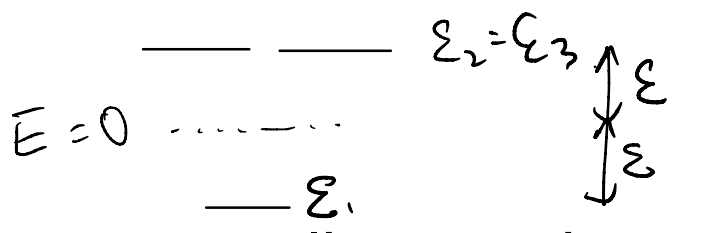
\includegraphics[width=\textwidth]{jupyterbook/data/fig/lec06-fig00.png}
\end{figure}

Without electron-phonon coupling, we have the eigen-energies

\begin{figure}[ht]
    \centering
    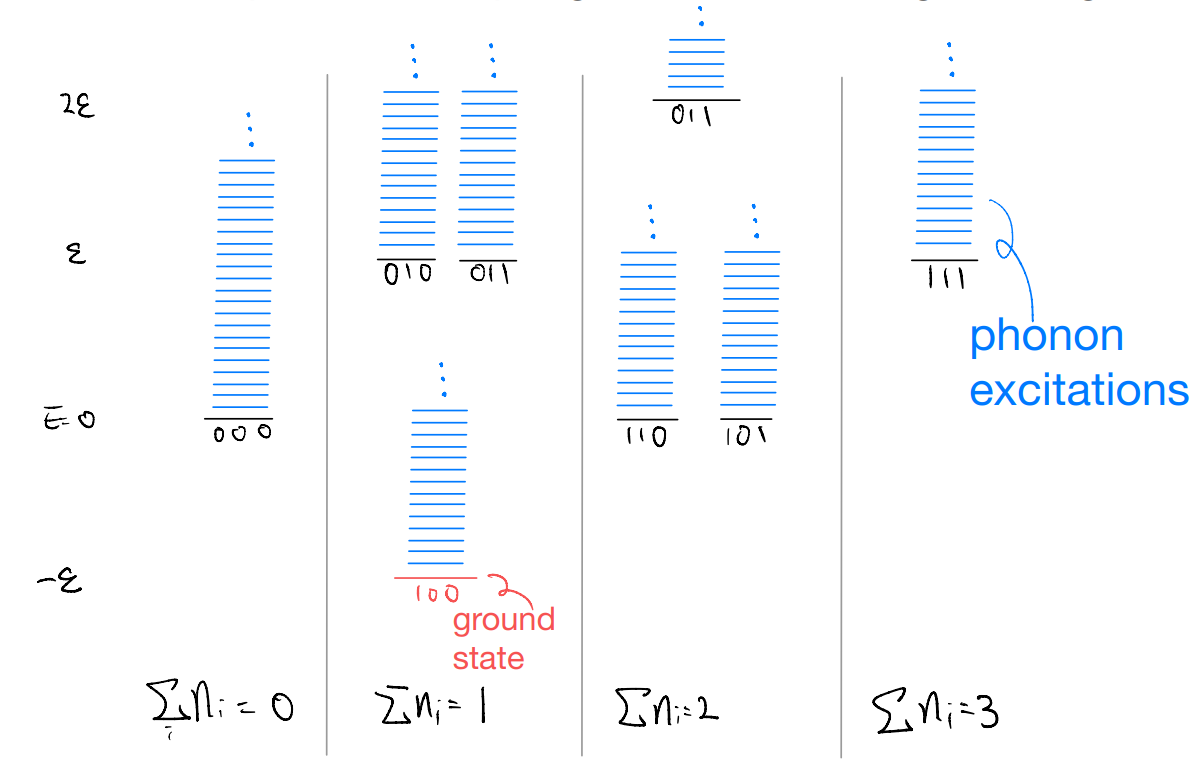
\includegraphics[width=\textwidth]{jupyterbook/data/fig/lec06-fig01.png}
\end{figure}

\noindent where for simplicity we considered an ``Einstein phonon'' model in which $\omega_q=\omega_E$ is $q$-independent. Otherwise, the phonon excitation should become a continuum as each mode (labeled by $q$) can have a different excitation energy.

Now, consider the effect of $\hat{H}_{e-ph}$, which we may treat as a perturbation to the level diagram above. A key simplifying assumption in our model (which enabled exact solutions) is that $[\hat{H},\hat{n}_i]=0$. In other words, even with the $e-ph$ coupling, we can think about each of the ``sub-block'' above individually.

\begin{figure}[ht]
    \centering
    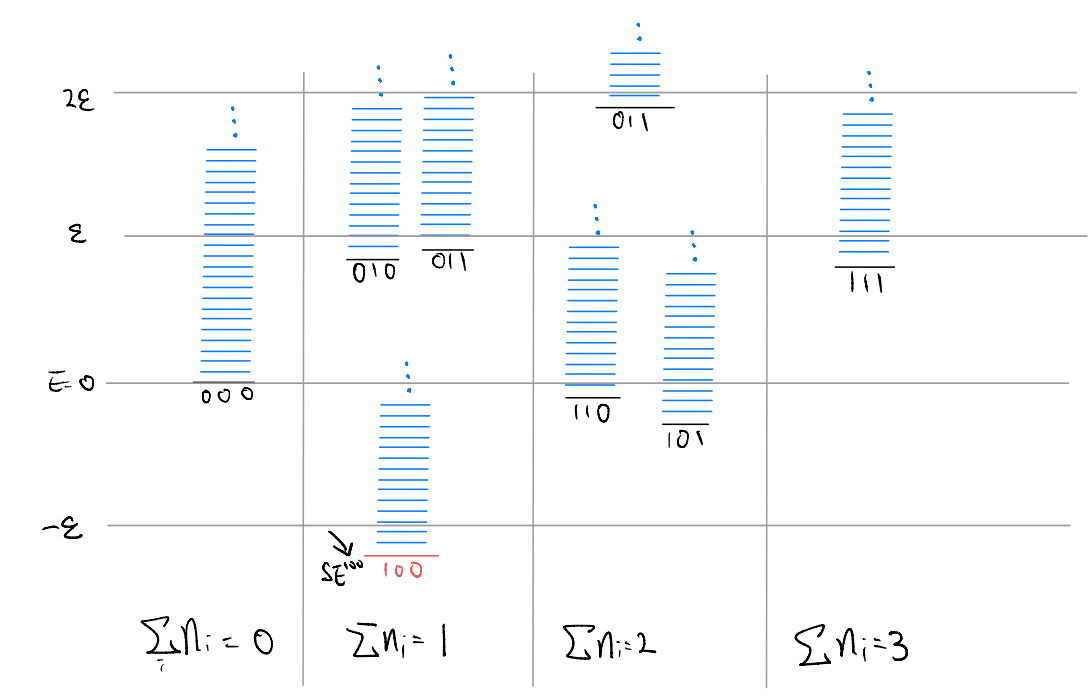
\includegraphics[width=\textwidth]{jupyterbook/data/fig/lec06-fig03.png}
\end{figure}

But this looks deceivingly simple! The phonon state $|\{m_q\} \rangle$ actually depends on the electronic occupation in a concealed manner. To see this more explicitly, let us write the Hamiltonian as
\begin{align*}
    \hat{H}=&\bigoplus_{\left\{ n_i \right\}}{\left. \hat{H} \right|_{\left\{ n_i \right\}}}\\
    =&\bigoplus_{\left\{ n_i \right\}}{\left( \sum_q{\hat{D}_{q}^{\dagger}\left( \frac{1}{\omega _q}\sum_i{n_iM_{iq}} \right) \omega _q\hat{a}_{q}^{\dagger}\hat{a}_q\hat{D}_q\left( \frac{1}{\omega _q}\sum_i{n_iM_{iq}} \right)}+\Delta \left( \left\{ n_i \right\} \right) \right)}
\end{align*}
where $\oplus$ is the direct sum over the $2^N$ independent sectors. It's still the ``same'' phonon Hamiltonian, but in different basis!

E.g., let $|\{m_q\}\rangle$ be the ``bare'' phonon eigenstates with phonon occupancy
\[ \hat{a}_{q}^{\dagger}\hat{a}_q\rightarrow m_q\]
Then the eigenstates of the Hamiltonian can be written as
\[ |\left\{ n_i \right\} ,\left\{ m_q \right\} \rangle =|\left\{ n_i \right\} \rangle \otimes \left[ \prod_q{\hat{D}_{q}^{\dagger}\left( \frac{1}{\omega _q}\sum_i{n_iM_{iq}} \right) |\left\{ m_q \right\} \rangle _0} \right] \]
Does this ``$i$-dependent basis rotation'' of the phonon matter? After all, the phonon energies are independent on the electronic configuration! The short answer is yes. To see why, we look into the electron's one-particle Green's function.

\section{Electron (impurity) Greens' function}

Let's look at a real-time one-particle Greens' function of the form
\[ G_{ii}\left( t \right) =-i\langle \Omega |\hat{c}_{i}^{\dagger}\left( t \right) \hat{c}_i\left( 0 \right) |\Omega \rangle \]
where $|\Omega \rangle$ is the ground state. We will compute $G_{ii}(t)$ in two ways
\begin{enumerate}
    \item Using the energy eigenstates we have derived. This is perhaps more transparent, but at the same time somewhat ``brute force'' and the solution approach looks a bit \emph{ad hoc}, since we cannot expect to solve the many-body Hamiltonian in general
    \item Solving the Heisenberg picture time evolution of the operator. This is probably the more systematic approach, and we will see that it allows for greater flexibility on the ground state
\end{enumerate}

Let us start with the ``brute force'' approach. For concreteness, we suppose the level scheme is the one drawn before, and so the ground state is
\[ |\Omega \rangle =|\left\{ 1,0,0 \right\} \rangle \otimes \prod_q{\hat{D}_{q}^{\dagger}\left( \frac{M_{1q}}{\omega _q} \right) |\left\{ 0_q \right\} \rangle _0}\]
\[ \hat{H}|\Omega \rangle =\Delta _{100}|\Omega \rangle \]
\[ \Delta _{100}=\varepsilon _1-\sum_q{\frac{M_{1q}^{2}}{\omega _q}}\]
